\section{Introduction}\label{sec:Intro}
Micro- and nano-robots can be manufactured in large numbers.
Our vision is for large swarms of robots remotely guided 1) through the human body, to cure disease, heal tissue, and prevent infection and 2) ex vivo to assemble structures in parallel. 
 For each application, large numbers of micro robots are required  to deliver sufficient payloads, but the small size of these robots makes it difficult to perform onboard computation.  Instead, these robots are often controlled by a global, broadcast signal. 
 The biggest barrier to this vision is a lack of control techniques that can reliably exploit large populations despite incredible under-actuation.  
 

\begin{figure}
\begin{center}
	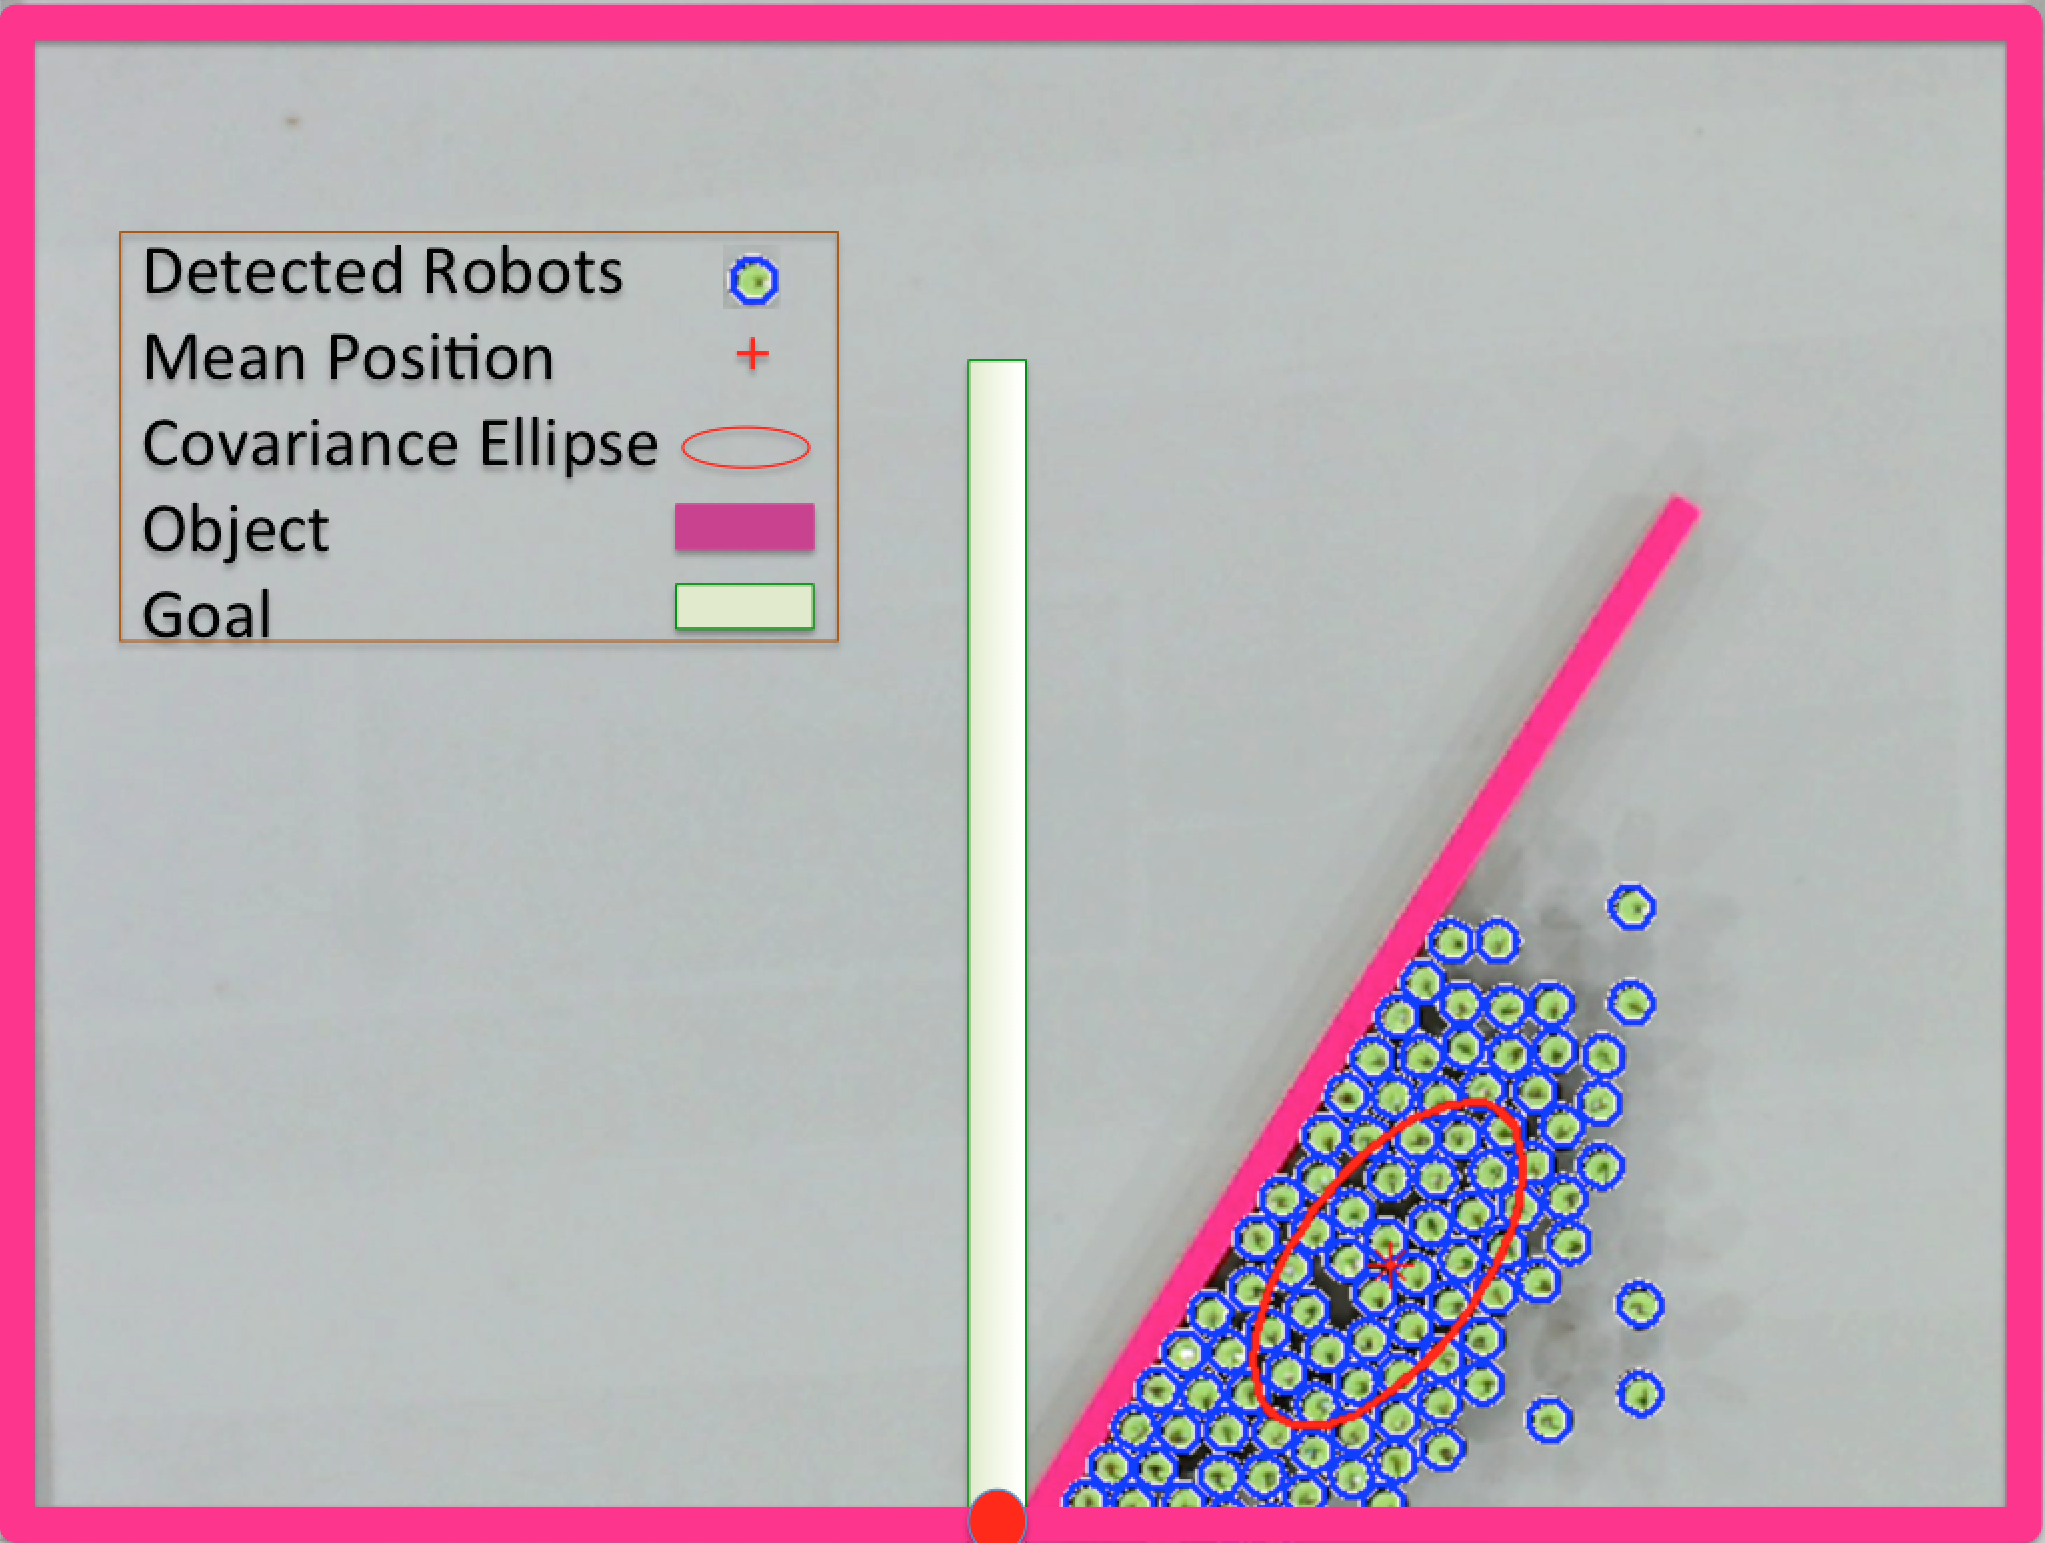
\includegraphics[width=.9\columnwidth]{FirstImage.png}
\end{center}
\vspace{-1em}
\caption{\label{fig:FirstImage}
Torque Control of an object is essential for manipulating objects to their goal position like when there is a narrow passageway . This paper shows how to apply force to get the required torque and force when we have a highly under-actuated system that all the robots are controlled globally with the same input. This figure shows 100 hardware robots apply torque to an object. These robots have light sensors and are programmed to go to the brightest light in the room which is their shared control input.
}
\vspace{-1em}
\end{figure}


%One surprising result was that humans that only knew the swarm's mean and covariance completed the task faster that humans who knew the position of every robot~\cite{Becker2013b}. Our previous work focused on a block-pushing task, where a swarm of robots pushed a larger block through a 2D maze. 
In previous work, we proved the mean position of a swarm is controllable and that, with an obstacle, the swarm's position variance orthogonal to rectangular boundary walls  is also controllable
($\sigma_x$ and $\sigma_y$ for a workspace with axis-aligned walls). 
The usefulness of these techniques was demonstrated by several automatic controllers. One controller steered a swarm of robots to push a larger block through a 2D maze~\cite{ShahrokhiIROS2015}. 
We also showed methods to control swarm's position covariance to be able to navigate the swarm through the workspaces with narrow corridors, but there is still another challenge remained. When the task is object manipulating, we need to control torque of the object also to successfully pass all the ways. 
This paper first discusses the ways that we can control torque of an object in Section ~\ref{sec:theory}. Then it introduces algorithms for torque control in Section ~\ref{sec:simulation}. We show that algorithms work in Section ~\ref{sec:expResults} on 100 kilobots.

%For controlling $\sigma_{xy}$, we prove that the swarm position covariance $\sigma_{xy}$ is controllable given boundaries with non-zero friction. 
%We then prove that two orthogonal boundaries with high friction are sufficient to arbitrarily position a swarm of $n$ robots. 
%We conclude by designing controllers that efficiently regulate $\sigma_{xy}$.


%This paper
%(1) proves that the swarm position covariance $\sigma_{xy}$ is controllable given boundaries with non-zero friction,  %where do we do this?
%(2) proves that two orthogonal boundaries with high friction are sufficient to arbitrarily position two robots, 
%(3) proves that two orthogonal boundaries with high friction are sufficient to arbitrarily position a swarm of $n$ robots, 
%(4) shows full-state position control with 2 or more robots using  extensive simulations, and
%(5) demonstrate covariance control on our hardware platform with a large number of hardware robots.
%TODO JOURNAL: design controllers that efficiently regulate $\sigma_{xy}$.
%TODO JOURNAL: We will design Lyapunov-inspired controllers for $\sigma_{xy}$ to prove controllability. 
%TODO JOURNAL:  and rank controllability as a function of friction.
% TODO: JOURNAL: and vary wall friction by laser-cutting boundary walls with a variety of profiles. 







% Our paper is organized as follows.  After a discussion of related work in Section \ref{sec:RelatedWork}, we describe our experimental methods for an online human-user experiment in Section \ref{sec:expMethods}.  We report the results of our experiments in Section \ref{sec:expResults}, discuss the lessons learned in Section \ref{sec:discussion}, and end with concluding remarks in Section \ref{sec:conclusion}.


